\documentclass[a4paper, headsepline]{scrartcl}
\usepackage[T1]{fontenc} % speziell für deutsch
\usepackage[english]{babel}
\usepackage[utf8]{inputenc}
\usepackage{hyperref}
\usepackage[pdftex]{graphicx}
\usepackage{tabularx, booktabs}
\usepackage{geometry}
\usepackage{scrpage2}
\usepackage{graphicx}
\usepackage{listings}
\usepackage{color}
\usepackage{lstautogobble}
\usepackage{float}
\usepackage{microtype} %verhindert zu breite Texte
\usepackage{setspace}
\usepackage{abstract}
\usepackage[justification=justified,singlelinecheck=false]{caption}
\usepackage[normalem]{ulem}
\useunder{\uline}{\ul}{}
\usepackage[toc,page]{appendix}


%Zeilenabstand
\onehalfspacing


%\restylefloat{figure}

 
%Seitenrandeinstellungen
%\geometry{top=12mm,left=25mm,right=25mm,bottom=13mm, includeheadfoot, headsep=12mm, foot=1cm}

%kein Einrücken nach Absaetzen
\setlength{\parindent}{0em} 


%Kopfzeileneinstellungen
\clearscrheadfoot 
%\pagestyle{scrheadings}  %linie unter Kopfzeile
%\automark[subsection]{section} 
%\renewcommand{\sectionmark}[1]{\markboth{#1}{}}% 
%\ihead{Federated Identities for Worldwide Scientific Collaboration\hfill\leftmark}
%\setheadsepline{0.2pt}
\setlength{\headheight}{1.1\baselineskip}

%Fusszeileneinstellung
\cfoot{\pagemark}
 
%kein Mensch will Boxen um Inhaltsverzeichnispunkte
\hypersetup{%
    pdfborder = {0 0 0}
}

%Zitierweise
\usepackage[backend=biber, style=ieee, natbib=true, hyperref=false,firstinits=true, bibencoding=utf8]{biblatex}
\renewcommand*{\labelnamepunct}{\addcolon\addspace}
\renewcommand*{\newunitpunct}{\addcomma\addspace}
\renewcommand*{\finentrypunct}{}
\DeclareFieldFormat{title}{#1\isdot}

%erzwingt Blocksatz auch wenn dadurch Lücken zwischen Wörtern entstehen
%nur wenn mans nicht anders will :)
%\sloppy

% Befehl für Anführungszeichen %Stefan: Wie folgt anwenden: \qte{Dieser Text ist in anführungszeichen}. Okay? Keine normalen Anführungszeichen reinschreiben
\newcommand{\qte}[1]{\glqq#1\grqq}
% \qte {Hase}

%Auch Paragraphen nummerieren und ins Inhaltsverzeichnis aufnehmen
\setcounter{secnumdepth}{4}  % = Nummerierung vertiefen *
\setcounter{tocdepth}{4}   %= Aufnahme in das Inhaltsverzeichnis *

%% ################# Listings ###################

\usepackage[section]{minted}


\graphicspath{{Pictures/}}

\bibliography{literatur}
%\bibliographystyle{plain}
	
\usepackage[babel,english]{csquotes}
%Diese Felder sollen nicht im Inhaltsverzeichnis angzeigt werden
\AtEveryBibitem {
	\clearlist{address}
	\clearfield{date}
	\clearfield{eprint}
	\clearfield{isbn}
	\clearfield{issn}
	\clearlist{location}
	\clearfield{month}
	\clearfield{series}
	\clearfield{edition}
	\clearfield{pagetotal}}
	
%% Einbinden der bib-Datei (=Quellen)
\bibliography{literatur.bib}
\begin{document}
	\pagenumbering{Roman}
	
	
	\begin{titlepage}
		\begin{center}
			
\includegraphics[scale=1.5]{Deckblatt/HTW_Logo_rgb.jpg} \qquad \qquad \\[4ex]
			\Large{\textbf{Web Applications}} \\[8ex]
			\LARGE{\textbf{Watering of Things}}\\[3ex]
			\large{\quad} \\ %Schriftgröße fürs Deckblatt definieren (wenn diese Zeile entfernt wird ist alles weitere in LARGE
			\begin{tabular}{l l l} \\
				Verfasser: & \quad Doreen Sacker, Tobias Wochinger \\[2ex]
				Studiengang: & \quad Internationale Medieninformatik (Master)\\
                 & \quad Angewandte Informatik (Master) \\[2ex]
				%Fachbereich: & \quad Wirtschaftswissnschaften II \\[2ex]
				Matrikelnummern: & \quad 552936, 552880 \\[2ex]
				Zuständiger Prof.: & \quad Prof. Dr. Gefei Zhang \\[2ex]
				%& \quad Yves Kemp \\[2ex]
				Datum: & \quad 01. Februar 2017 %\quad (Ver. 1.03)
			\end{tabular}
		\end{center}
	\end{titlepage}
	\newpage
	\tableofcontents
	\newpage
	\pagenumbering{arabic}
    \section{Einleitung}
Nachdem JavaScript früher überwiegend bei der Entwicklung im Frontend zum Einsatz kam, profitieren JavaScript-Entwickler immer mehr vom Paradigma \textit{Learn once, write anywhere}. So schickt sich JavaScript an, mit dem Boom von NodeJS auch serverseitig verstärkt eine Rolle zu spielen. Mobile Applikationen konnten jedoch bisher nur eingeschränkt mittels JavaScript umgesetzt werden. Zu groß waren die Limitierungen durch den Fakt, dass mit JavaScript erstellte Applikationen nur innerhalb einer Web-View auf den Geräten ausgeführt werden konnten. Auf einem Hackathon entwickelte Facebook jedoch 2013 eine Möglichkeit React-Komponenten durch native UI-Komponenten auf den Geräten zu visualisieren. Dieser Prototyp wurde daraufhin innerhalb interner Projekte bei Facebook weiterentwickelt, bis eine erste Version von React Native schließlich im März 2015 als Open-Source-Projekt veröffentlicht wurde. Facebook hatte bei der Entwicklung ursprünglich lediglich die iOS-Plattform im Blick. Rasch wurde jedoch die Möglichkeit der Wiederverwendung für Android erkannt, sodass React Native seit Sptember 2015 auch für Android verfügbar ist.
Die Bereitstellung von React Native als Open-Source-Projekt sorgte von Beginn an für eine große Community, die React Native seitdem unter Facebooks Schirmherrschaft in großen Schritten vorantreibt. Über 9000 Commits von mehr als 1000 Entwicklern sowie ein zweiwöchiger-Release-Rhythmus zeugen von dem Bedarf und dem Potenzial der  Entwicklung nativer Smartphone-Applikationen mittels JavaScript.
    \section{Use Cases} \label{sec:usecases}
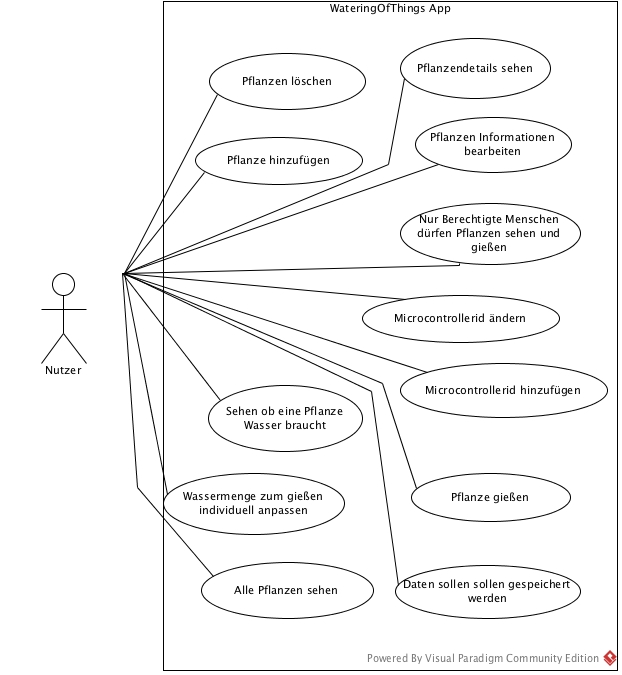
\includegraphics[scale=0.5]{usecase.jpg} \qquad \qquad \\[4ex]
    \section{Konzept}
    \subsection{Architektur}
    WateringOfThings besteht aus aus vier Haupt-Komponenten: 
   \begin{itemize}
       \item Microcontroller
           \begin{itemize}
               \item Bewässern der Pflanzen
               \item Erheben der Feuchtigkeitswerte der Blumenerde
           \end{itemize}
       \item MQTT-Broker
           \begin{itemize}
               \item Bidirektionale, leichtgewichtige Kommunikation zwischen Server und Microcontroller
               \item Informiert Server über Daten der Microcontroller
               \item Informiert ausgewählten Microcontroller über Befehle vom Server
           \end{itemize}
       \item Server
           \begin{itemize}
               \item Informiert Microcontroller in regelmäßigen Abständen die Feuchtigkeitswerte zu nehmen
               \item Speicherung aller Daten (Pflanzen, Feuchtigkeitswerte) in SQLite-Datenbank
               \item Bereitstellung aller Daten im JSON-Format via REST API
           \end{itemize}
    \item App
        \begin{itemize}
            \item Eingabeschnittstelle für Nutzer
            \item Visualisierung der Informationen
        \end{itemize}
   \end{itemize}
    \begin{figure}[H]
        \centering
        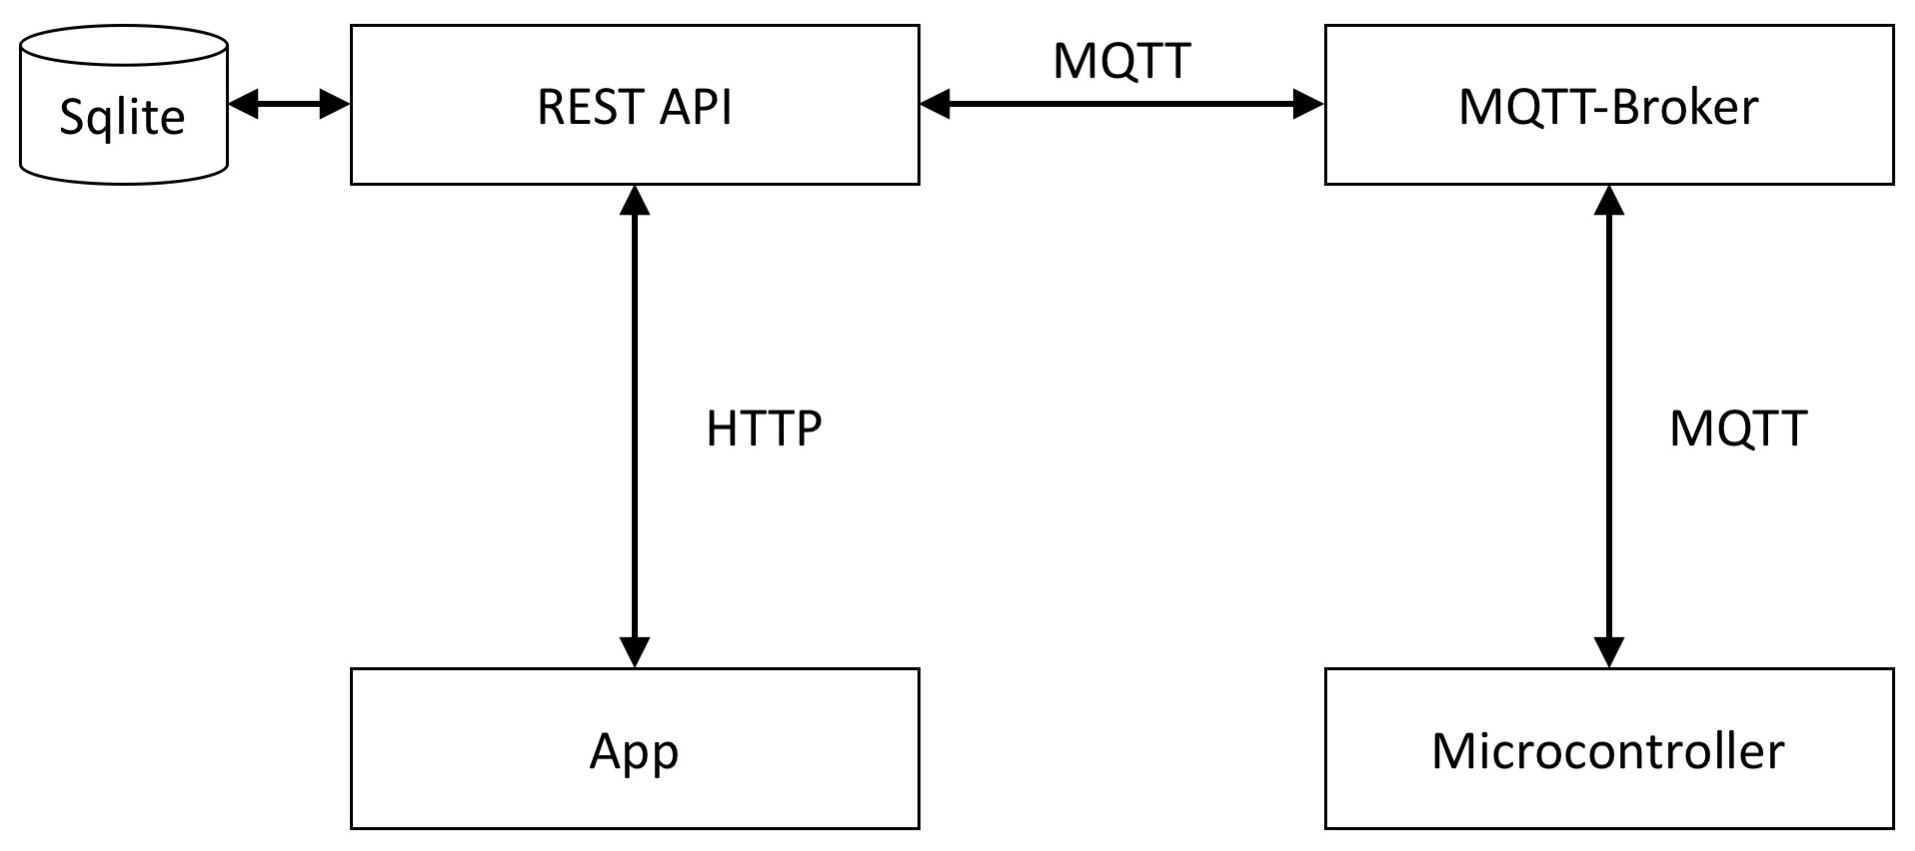
\includegraphics[width=0.7\linewidth]{../Pictures/Konzept/Architecture}
        \caption{Projektarchitektur}
        \label{fig:architecture}
    \end{figure}
    
    \subsection{Datenmodell} \label{ssec:datamodel}
    
     \begin{minipage}{\textwidth}
        Microcontroller\\
        \begin{tabularx}{\linewidth}{|l|l|X|}
            \hline
            Attribut & Datentyp & Beschreibung\\
            \hline
            id & String & Eindeutiger, sicherer Token zur Authentifizierung des Microcontrollers \\
            \hline                              
        \end{tabularx}
    \end{minipage}

\vspace{0.5cm}

     \begin{minipage}{\textwidth}
        Plant\\
          \begin{tabularx}{\linewidth}{|l|l|X|}
              \hline
            Attribut & Datentyp & Beschreibung\\
            \hline
            id & Int & Eindeutige ID der Pflanze \\
            name & String & Frei wählbarer Name für die Pflanze \\
            pin & Int & \begin{tabular}[t]{@{}ll}
            Pin am Microcontroller über den der \\Feuchtigkeitssensor verbunden ist \\
            \end{tabular}\\
            position & Int & Position der Pflanze in der Aufstellung in Grad \\
            moistureTreshold & Float & Wert unterhalb dessen die Pflanze als trocken gilt \\
            latestMoistureValue & Float & Letzter gemessener Feuchtigkeitswert der Pflanze  \\
            \hline                              
        \end{tabularx}
    \end{minipage}

\vspace{0.5cm}

     \begin{minipage}{\textwidth}
        MoistureValue\\
        \begin{tabularx}{\linewidth}{|l|l|X|}
            \hline
            Attribut & Datentyp & Beschreibung\\
            \hline
            date & Long & Timestamp, wann der Wert erhoben wurde \\
            value & Float & Erhobener Feuchtigkeitswert \\
            \hline                              
        \end{tabularx}
    \end{minipage}
    
    \subsection{Mobile Applikation}

        \subsubsection{React Native}
Ziel dieser Applikation ist es Nutzern eine einfache Möglichkeit zu geben, ihre Pflanzen auch im Urlaub versorgen zu können. Um möglichst viele Nutzer mit dieser App zu erreichen, wird eine Entwicklung für die Android- als auch für die iOS-Plattform angestrebt. Um nicht für beide Plattformen eine eigene App entwickeln zu müssen und damit den doppelten Entwicklungsaufwand zu haben, wurde eine Cross-Plattform angestrebt. Die Technologie, welche dies mit nativen Komponenten am besten vereint, ist React Native.
        
        \subsubsection{Views}\label{views}
Die WateringOfThings App besteht aus fünf verschiedenen Ansichten, Views. Diese führen den Nutzer durch die Anwendung und setzen die in Kapitel \ref{sec:usecases} beschriebenen Use Cases um. \\

Beim ersten Start der App wird der Nutzer nach der Eingabe einer Microcontroller-ID gefragt, wie in View \ref{microcontroller} zu sehen. Diese kann von der Hardwarekomponente abgelesen werden. Die Microcontroller-ID wird daraufhin von der App gespeichert. Der Nutzer kann die ID jeder Zeit unter dem Punkt \textit{Settings} ändern. Der erste View und der Settingsview sind dabei gleich. Zu jedem Microcontroller kann der Nutzer anschließend Pflanzen hinzufügen.  
\begin{figure}[H]
    \centering
    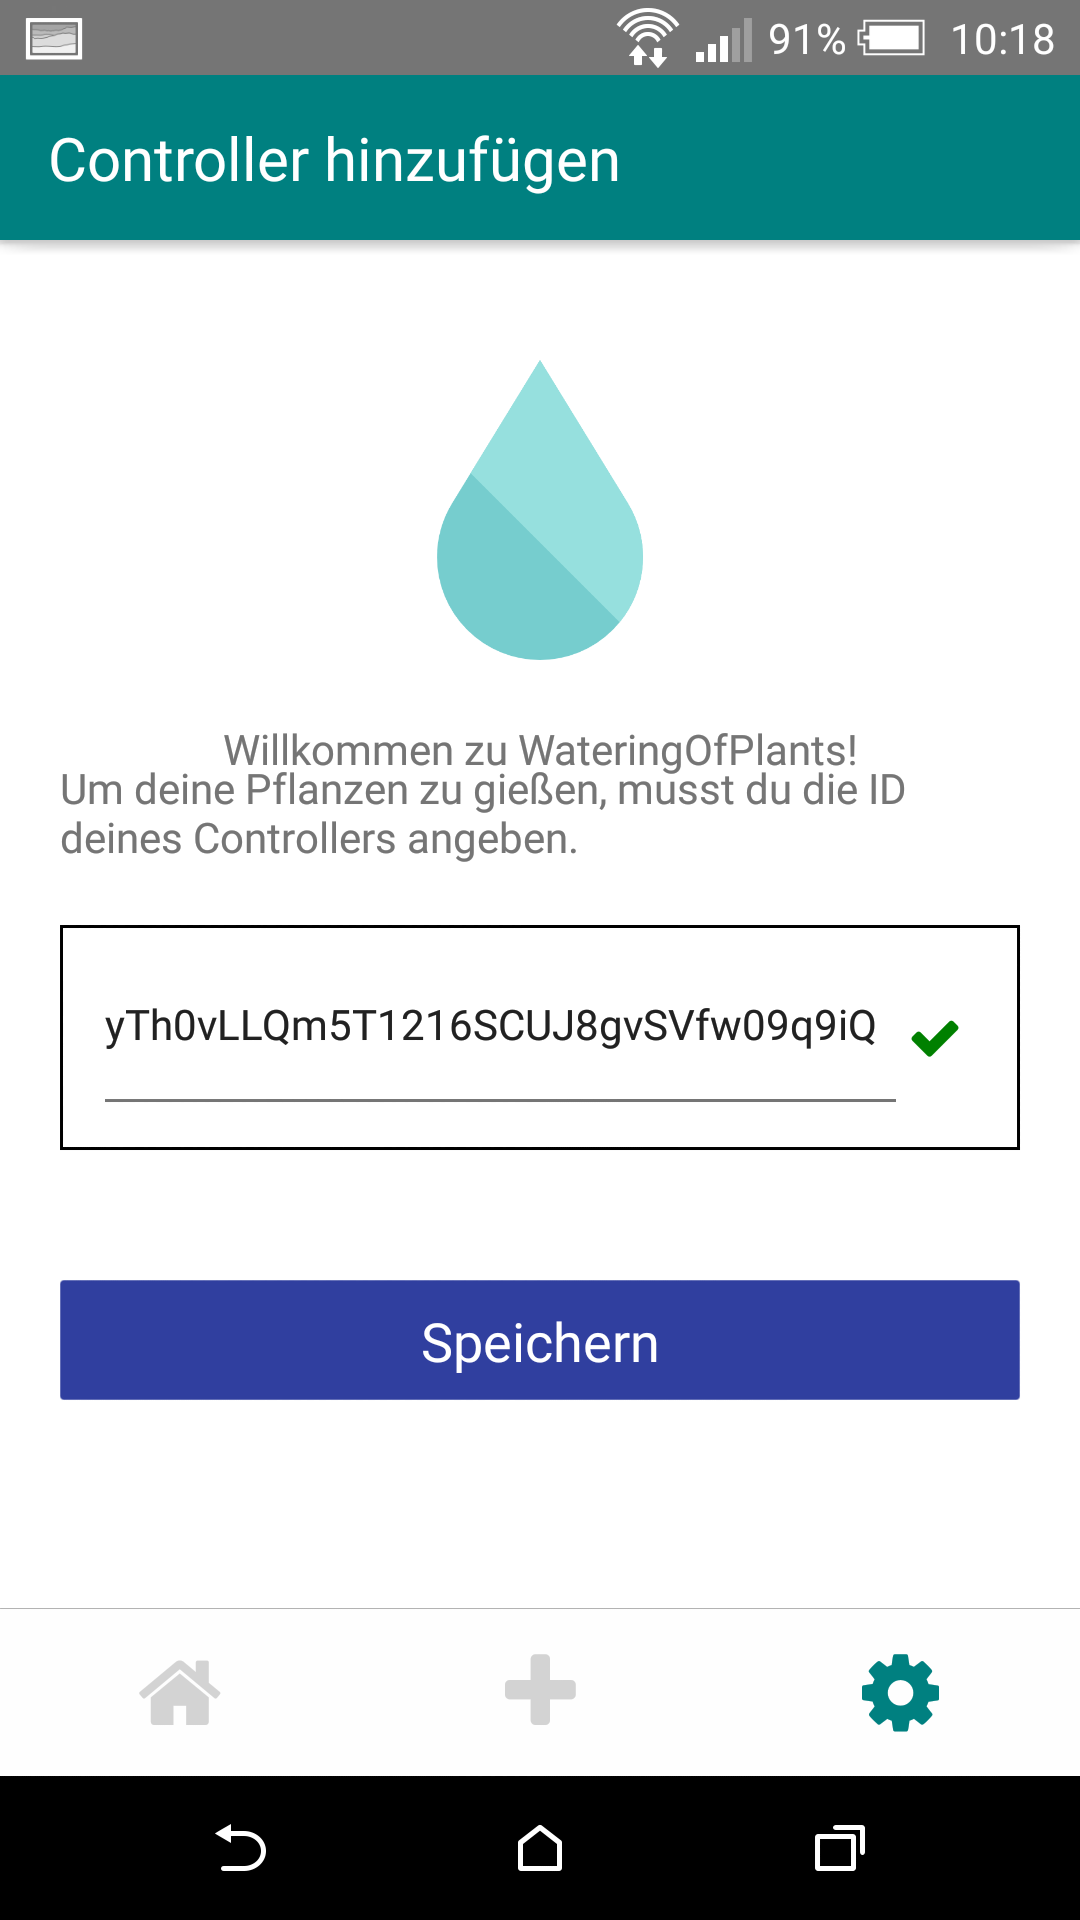
\includegraphics[scale=0.15]{Views/microcontroller.png}
    \caption{Hinzufügen der Microcontroller-ID}
    \label{microcontroller}
\end{figure}

Der Nutzer hat die Möglichkeit zu einer Microcontroller-ID Pflanzen hinzuzufügen, wie in View \ref{add}. Hierzu kann der Nutzer ein eigenes Bild der Pflanze aus der Galerie seiner gespeicherten Fotos auswählen. Wird kein Bild ausgewählt wird ein Standardbild angezeigt. Für die Pflanze kann ein Name vergeben werden, z.B. Basilikum. Der Pin ist der Anschluss am Microcontroller. Über ihn kann der Feuchtigkeitssensor mit der Pflanze verbunden werden. Da die Pflanzen in einem Halbkreis um den Microcontroller aufgestellt werden, muss die Position angegeben werden. Diese wird in Grad eingegeben. Weitere Information sind im Datenmodell (siehe Kapitel \ref{ssec:datamodel}) zu finden. \\

Des Weiteren kann ein Trockenheitsschwellwert für die Pflanze angegeben werden. Jede Pflanze braucht unterschiedlich viel Wasser. Um bestimmen zu können, wann eine Pflanze das nächste mal gegossen werden sollte, ist der Schwellwert einstellbar. Braucht eine Pflanze wenig Wasser, wie zum Beispiel ein Kaktus, wird der Slider weiter nach links bewegt. Braucht die Pflanze mehr Wasser, wird der Slider nach rechts bewegt. \\

Über eine Validierung wird sichergestellt, dass der Nutzer nur valide Eingaben machen kann. Ist die Eingabe nicht valide, wird ein rotes Ausrufezeichen angezeigt. Ist die Eingabe valide wird ein grüner Haken angezeigt. Erst wenn alle Eingaben valide sind, kann die Pflanze gespeichert werden. 

\begin{figure}[H]
    \centering
    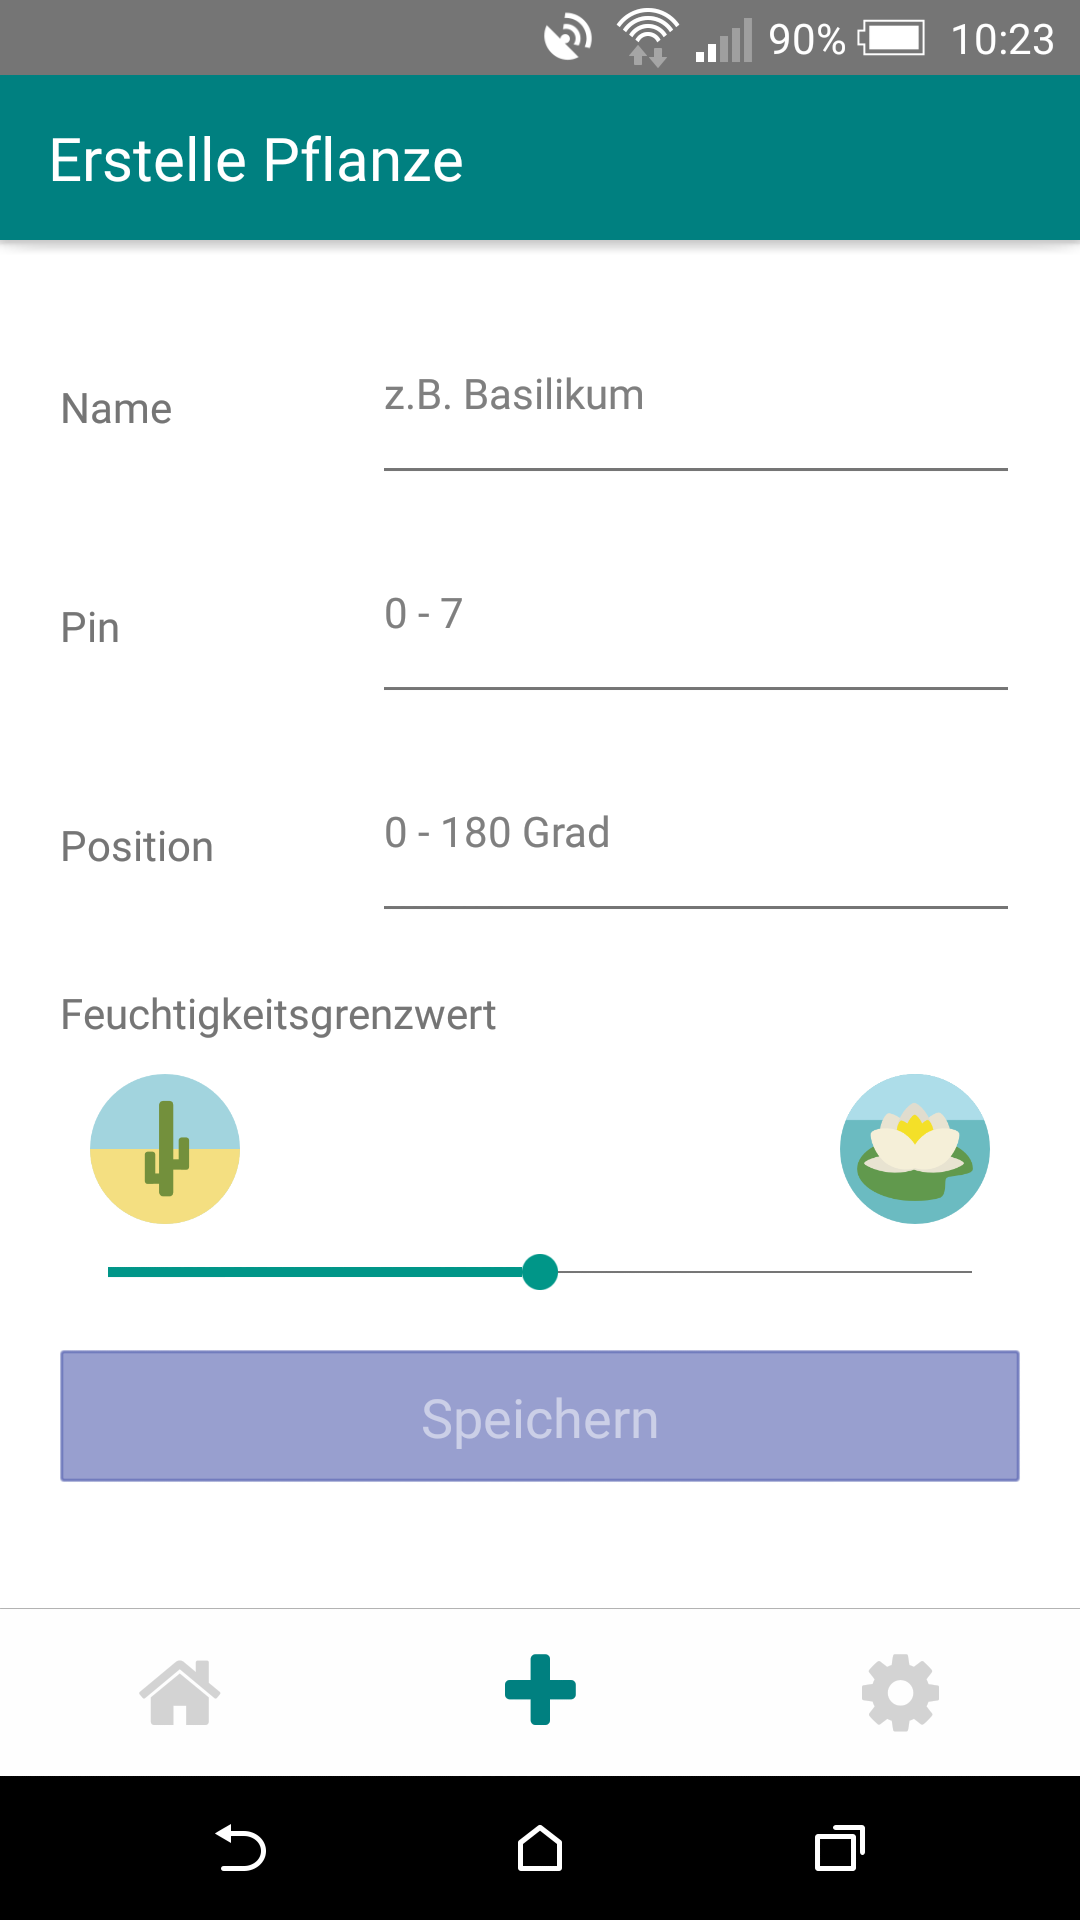
\includegraphics[scale=0.15]{Views/add.png}
    \caption{Pflanze hinzufügen}
    \label{add}
\end{figure}

Alle Pflanzen werden, wie in Abbildung \ref{list} gezeigt,  in einer Liste dargestellt. Die Pflanzen werden vom Nutzer zu einer bestimmten Microcontroller-ID hinzugefügt. Der View teilt sich in zwei Listen, eine für zu trockene Pflanzen und eine für gut bewässerte Pflanzen. Fällt der gemessene Feuchtigkeitswert einer Pflanze unter ihren Schwellwert, wird die Pflanze in der Liste für Pflanzen angezeigt, die zu trocken sind. Dem Nutzer ist mithilfe der Listen schnell ersichtlich, welche Pflanzen gegossen werden sollten und kann selbst entscheiden, wann der beste Zeitpunkt ist. Die Pflanzen werden mit ihrem gespeicherten Bild angezeigt, ist kein Bild gespeichert, wird ein Standardbild angezeigt. In der oberen Navigationsleiste wird der Name der App mit Logo dargestellt. Zusätzlich hat man in der Navigation die Möglichkeit eine Pflanze hinzuzufügen. Die untere Tableiste ist in allen Views gleich. Der Nutzer kann mit \textit{Home} stets zur Listenansicht zurück navigieren. Mit dem Tab \textit{Add} kann der Nutzer eine neue Pflanze anlegen und im \textit{Settings}-Tab die Microcontroller-ID ändern.
\begin{figure}[H]
    \centering
    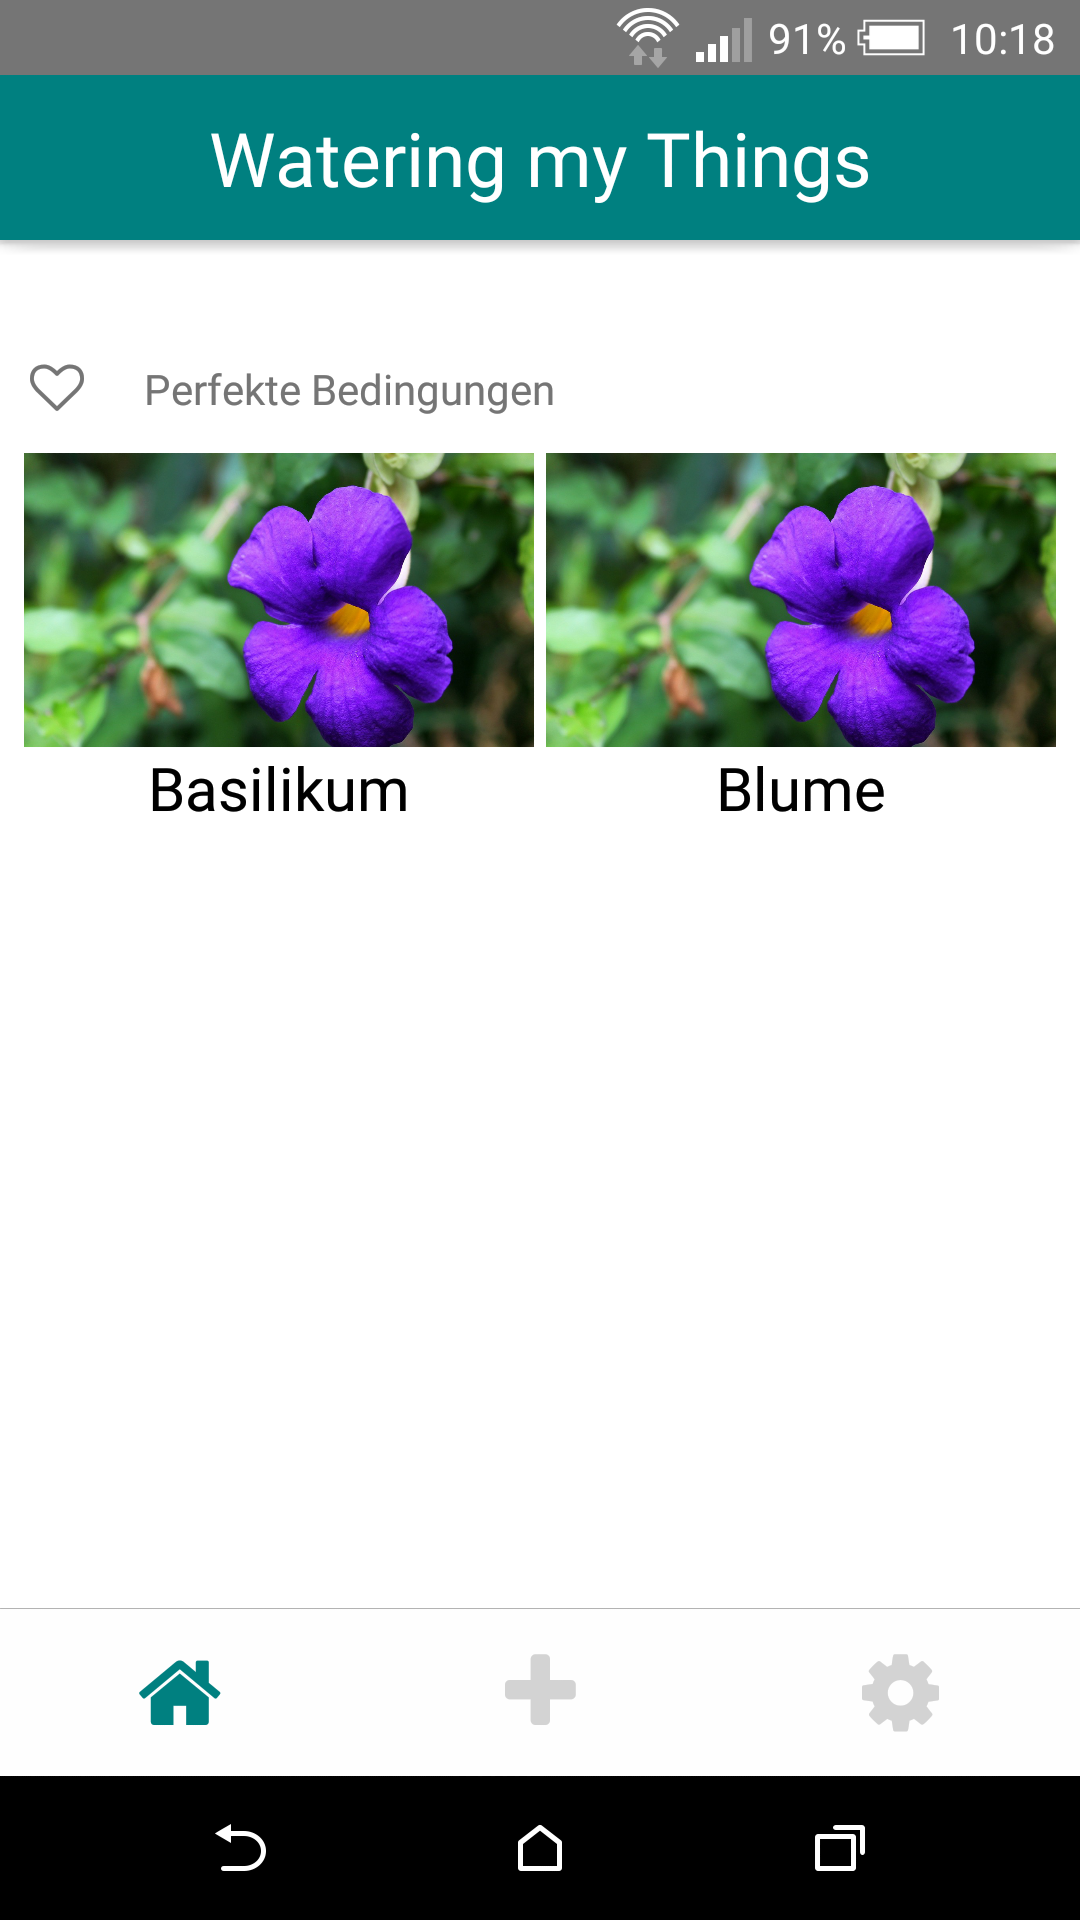
\includegraphics[scale=0.15]{Views/list.png}
    \caption{Liste der Pflanzen}
    \label{list}
\end{figure}

Der Nutzer hat die Möglichkeit eine Pflanze aus der Liste auszuwählen und auf eine View mit Detailinformationen (siehe Abbildung \ref{fig:plantview}) weitergeleitet zu werden. Auf der Detailseite für die einzelnen Pflanzen wird der Feuchtigkeitsstatus der Pflanze genauer angezeigt. Der Name der Pflanze wird oben in Navigation angezeigt. Rechts davon hat der Nutzer mit dem Änderungs-Icon die Möglichkeit die Daten der Pflanze zu bearbeiten. Für die Bearbeitungs-View wird die Erstellungsview wiederverwendet.\\

Über den \textit{Water}-Button hat der Nutzer die Möglichkeit eine Pflanze zu gießen. Hierfür wird er auf die in Abbildung \ref{fig:watering} gezeigte View weitergeleitet. In dieser View zum Gießen der Pflanze sieht man noch einmal den Feuchtigkeitsstatus der Pflanze. Weiter hat man die Möglichkeit die Wassermenge zu bestimmen mit der die Pflanze gegossen werden soll. 

\begin{figure}[]
    \centering
    \begin{minipage}[b]{0.4\textwidth}
        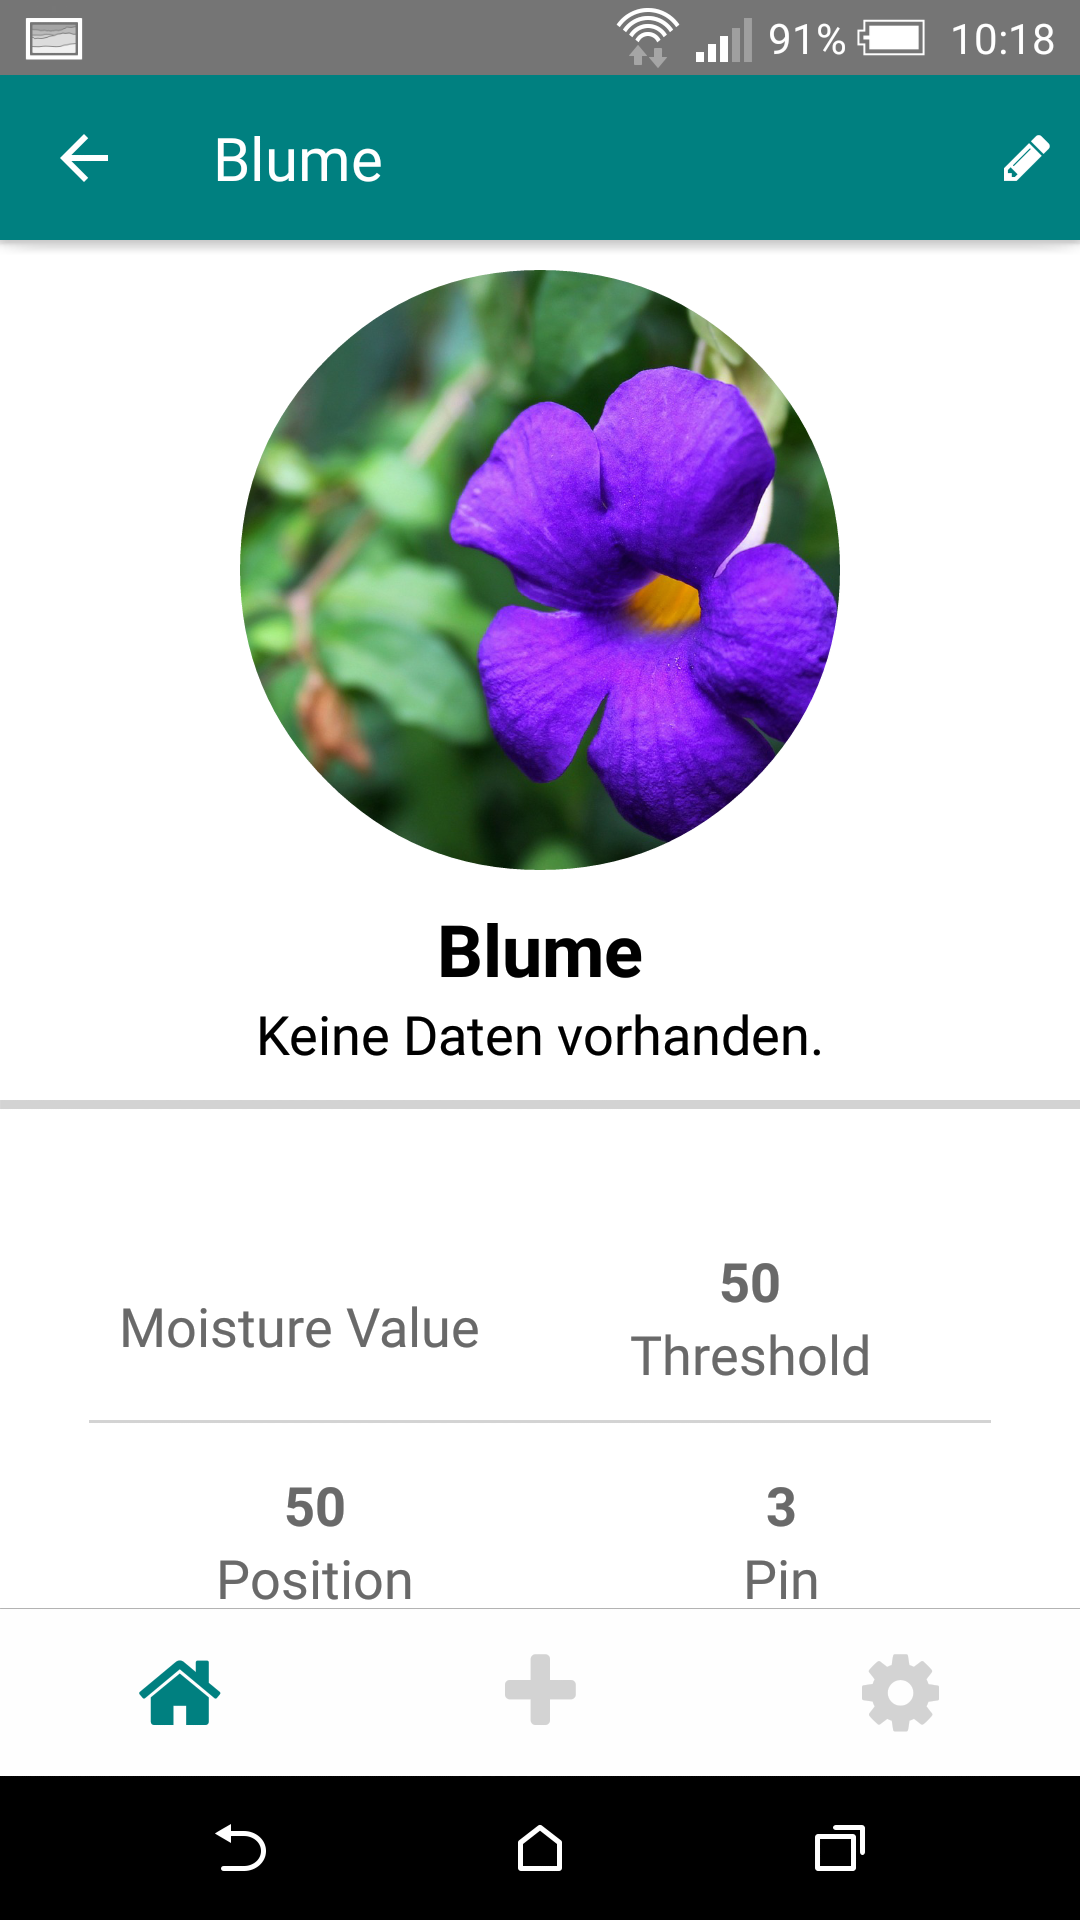
\includegraphics[scale=0.15]{Views/plant.png}
        \caption{Detailseite einer Pflanze}
        \label{fig:plantview}
    \end{minipage}
    \hfill
    \begin{minipage}[b]{0.4\textwidth}
        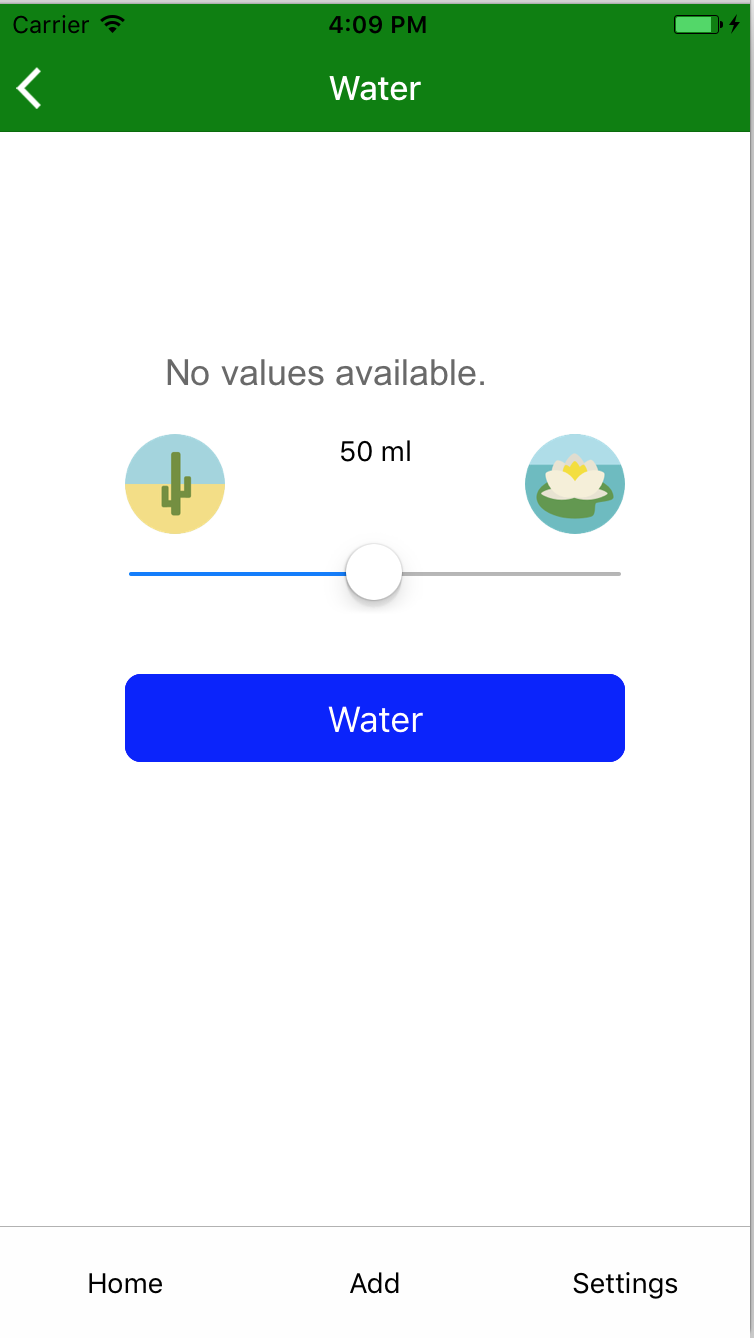
\includegraphics[scale=0.15]{Views/water.png}
       \caption{Pflanze gießen}
       \label{fig:watering}
    \end{minipage}
\end{figure}



    \subsection{Server}

        \subsubsection{REST API}
        Auf dem Server läuft eine Webapp, welche mit dem Python Web Application Framework \textit{Django} umgesetzt wurde. Django bietet im Gegensatz zu Alternativen, wie \textit{Flask}, schon eine große Vielfalt an Funktionalität Out-of-the-Box an. Nützlich erweist sich hierbei insbesondere das ORM-Mapping, welches den Umgang mit der Datenbank sehr einfach macht sowie es ermöglicht die verwendete Datenbank ohne Aufwand zu ändern. Aktuell wird als Datenbank \textit{SQLite} genutzt. Falls diese bei steigender Nutzeranzahl nicht mehr ausreicht, kann durch bloße Änderung der Verbindungsdaten auf andere Datenbanken, wie \textit{MySQL} oder \textit{MongoDB}, gewechselt werden.
        Folgenden weiteren Frameworks / Bibliotheken werden genutzt:
        \begin{itemize}
            \item django-rest-framework: Bereitstellung der REST-API
            \item paho-mqtt: Kommunikation mit dem MQTT-Broker
            \item celery: Asynchrones, periodisches Beauftragen der Feuchtigkeitsmessungen
        \end{itemize}
    
        \subsubsection{Ressourcen}
        Die Daten werden als JSON und XML bereitgestellt. Die angegebene URL stellt jeweils den dynamischen Teil der URL dar. Diese wird dem festen Teil der URL angehängt, welcher die Form \textit{https://<host>:<port>/api/v\{n\}/} hat. Die eincodierte Versionsnummer der API ermöglicht es, verschiedene Versionen der API parallel zu betreiben.\\
        
        \newcommand{\tabitem}{~~\llap{\textbullet}~~}
     \begin{minipage}{\textwidth}
             GET controller/\{controllerID\}/ 
        
          \begin{tabularx}{\textwidth}{lX}
                \toprule Beschreibung & Überprüft Validität der Controller-ID \\
                URL-Parameter & controllerID: zu überprüfende ID des Controllers \\
                Body & - \\
                Response & \{ "exists": true/false\}
            \end{tabularx}
    \end{minipage}\\\\
        
     \begin{minipage}{\textwidth}
            GET controller/\{controllerID\}/plant/ 

          \begin{tabularx}{\textwidth}{lX}
                \toprule Beschreibung & Alle Pflanzen des Microcontrollers \\
                URL-Parameter & controllerID: ID des Controllers mit dem die Pflanzen verbunden sind \\
                Body & - \\
                Response & Liste von Pflanzen
            \end{tabularx}
    \end{minipage}\\\\
        
     \begin{minipage}{\textwidth}
             POST  controller/\{controllerID\}/plant/ 
         
          \begin{tabularx}{\textwidth}{lX}
             \toprule Beschreibung & Erstellt eine neue Pflanze \\
             URL-Parameter & controllerID: ID des Controllers mit dem die Pflanzen verbunden sind \\
             Body & Zu erstellende Pflanze ohne ID \\
             Response & Erstellte Pflanze mit ID
         \end{tabularx}
    \end{minipage}\\\\
     
     \begin{minipage}{\textwidth}
              GET  controller/\{controllerID\}/plant/\{plantID\}/
          
          \begin{tabularx}{\textwidth}{lX}
              \toprule Beschreibung & Alle Informationen zu einer spezifischen Pflanze \\
              URL-Parameter & 
                  \begin{tabular}[t]{ll}
                       \tabitem controllerID: ID des Controllers mit dem die Pflanzen verbunden sind \\ 
                       \tabitem plantID: Eindeutige ID der angefragten Pflanze
                  \end{tabular}\\
              Body & - \\
              Response & Pflanzenobjekt
          \end{tabularx}
    \end{minipage}\\\\
          
     \begin{minipage}{\textwidth}
              PUT controller/\{controllerID\textgreater/plant/\{plantID\}/
          
            \begin{tabularx}{\textwidth}{lX}
              \toprule Beschreibung & Updated eine existierende Pflanze \\
              URL-Parameter & 
              \begin{tabular}[t]{ll}
                  \tabitem controllerID: ID des Controllers mit dem die Pflanzen verbunden sind \\ 
                  \tabitem plantID: Eindeutige ID der zu updatenden Pflanze
              \end{tabular}\\
              Body & Geändertes Pflanzenobjekt \\
              Response & Geändertes Pflanzenobjekt
          \end{tabularx}
    \end{minipage}\\\\
      
     \begin{minipage}{\textwidth}
         
              DELETE controller/\{controllerID\}/plant/\{plantID\}/ 
          
          \begin{tabularx}{\textwidth}{lX}
              \toprule Beschreibung & Löschen einer Pflanze \\
              URL-Parameter & 
              \begin{tabular}[t]{ll}
                  \tabitem controllerID: ID des Controllers mit dem die Pflanzen verbunden sind \\ 
                  \tabitem plantID: Eindeutige ID der zu löschenden Pflanze
              \end{tabular}\\
              Body & - \\
              Response & -
          \end{tabularx}
        \end{minipage}\\\\
      
     \begin{minipage}{\textwidth}
         
              GET  controller/\{controllerID\}/plant/\{plantID\}/moisture/
          
          \begin{tabularx}{\textwidth}{lX}
              \toprule Beschreibung & Abfragen aller Feuchtigkeitsmessungen für eine Pflanze \\
              URL-Parameter & 
              \begin{tabular}[t]{ll}
                  \tabitem controllerID: ID des Controllers mit dem die Pflanzen verbunden sind \\ 
                  \tabitem plantID: Eindeutige ID der Pflanze
              \end{tabular}\\
              Body & - \\
              Response & Liste an Feuchtigkeitswerten
          \end{tabularx}
        \end{minipage}\\\\
      
     \begin{minipage}{\textwidth}
             
      POST controller/\{controllerID\}/plant/\{plantID\}/water/\{amount\}/
      
          \begin{tabularx}{\textwidth}{lX}
          \toprule Beschreibung & Bewässerung einer Pflanze \\
          URL-Parameter & 
          \begin{tabular}[t]{ll}
              \tabitem controllerID: ID des Controllers mit dem die Pflanzen verbunden sind \\ 
              \tabitem plantID: Eindeutige ID der zu bewässernden Pflanze \\
              \tabitem amount: Wassermenge in Millilitern
          \end{tabular}\\
          Body & - \\
          Response & -
      \end{tabularx}
  \end{minipage}\\

    \subsection{Microcontroller}

        \subsubsection{Kommunikation}
        Zur Kommunikation wird das Protokoll \textit{MQTT} verwendet. MQTT ist ein leichtgewichtiges Nachrichtenprotokoll, welches auf TCP/ IP aufbaut. Es wurde speziell für Anwendungen mit geringen Ressourcen sowie für limitierten Bandbreite entworfen. Damit eignet es sich sehr gut für Internet-of-Things-Anwendungen, wird aber auch zunehmend bei mobilen Applikationen genutzt.
        
        MQTT setzt das \textit{Publish-Subscribe-Pattern} um. Server und Microcontroller sind beide Clients, die sich mit einem gemeinsamen MQTT-Broker verbinden. Dort können sie sich für Benachrichtigungen zu speziellen Themen anmelden (\textit{subscribe}). Themen werden als URL dargestellt. Inhalte zu einem Thema können veröffentlicht (\textit{publish}) werden. Der Broker benachrichtigt dann automatisch alle Clients, welche sich für das Thema eingeschrieben haben.
        
        Die Form der gesendeten Daten unterscheidet sich teilweise etwas vom gewohnten Vorgehen mit leistungsstärkeren Geräten. Die Form ist darauf ausgelegt zu jeder Zeit eine minimale Menge an Daten auf dem Microcontroller vorzuhalten sowie diese möglichst leichtgewichtig lesbar zu machen.\\
        
        \begin{minipage}{\textwidth}
            WateringOfPlants/microController/\{controllerID\}/water
            
            \begin{tabularx}{\textwidth}{lX}
                \toprule Beschreibung & Anweisung vom Server eine Pflanze zu bewässern  \\
                URL-Parameter & controllerID: ID des Controllers der die Pflanze bewässern soll\\
                Daten & 
                  \begin{tabular}[t]{ll}
                      \{ \\
                          \tab "position": <position>, \\
                          \tab "time": <time> \\
                      \} \\
                    \tabitem position: Position der Pflanze in Grad \\ 
                    \tabitem time: Zeit in Millisekunden für die die Pumpe aktiviert werden soll
                \end{tabular}\\
            \end{tabularx}
        \end{minipage}\\\\
        
        \begin{minipage}{\textwidth}
            WateringOfPlants/microController/\{controllerID\}/measure
                    
            \begin{tabularx}{\textwidth}{lX}
                \toprule Beschreibung & Anweisung vom Server die Feuchtigkeitswerte zu erheben  \\
                URL-Parameter & controllerID: ID des Controllers, der die Werte erheben soll\\
                Daten & 
                \begin{tabular}[t]{ll}
                    \{ \\
                    \tab "pins": [<pinNr>, <pinNr> ... ]>, \\
                    \tab "nrOfPins": <nrOfPins> \\
                    \} \\
                    \tabitem pins: Pins an denen die Feuchtigkeitssensoren angeschlossen sind \\ 
                    \tabitem nrOfPins: Länge des pins-Arrays
                \end{tabular}\\
            \end{tabularx}
        \end{minipage}\\\\
        
        \begin{minipage}{\textwidth}
            WateringOfPlants/microController/\{controllerID\}/measuredValues/\{pinNr\}
            
            \begin{tabularx}{\textwidth}{lX}
                \toprule Beschreibung & Gemessener Feuchtigkeitswert vom Microcontroller  \\
                URL-Parameter &  
                \begin{tabular}[t]{ll}
                    \tabitem controllerID: ID des Controllers, der den Feuchtigkeitswert erhoben hat.\\ 
                    \tabitem pinNr: Pin, zu welchem der Feuchtigkeitswert erhoben wurde
                \end{tabular}\\
                Daten & 
                \begin{tabular}[t]{ll}
                    <moistureValue> \\
                    \tabitem moistureValue: Erhobener Feuchtigkeitswert als Double
                \end{tabular}\\
            \end{tabularx}
        \end{minipage}\\
    
        \subsubsection{Aufbau}
        Die Möglichkeit einer Tröpfchenbewässerung wurde verworfen, um größere Unterschiede bei der Pflanzenbewässerung sicherstellen zu können. Um trotzdem möglichst viele Pflanzen versorgen zu können, wird ein halbkreisförmiger Aufbau der Pflanzen vorausgesetzt, wie in Abbildung \ref{fig:position} gezeigt. Damit können von einer Hardwarekomponente fünf Pflanzen versorgt werden. \\
        
        Für den Aufbau werden folgende Komponenten mindestens benötigt:
        \begin{itemize}
            \item 1 WLAN-fähiger Microcontroller, der mittels MQTT kommunizieren kann
            \item 1 Wasserquelle, z.B. ein Eimer
            \item 1 Wasserschlauch über den das Wasser von der Quelle zur Pflanze geleitet wird
            \item 1 Servomotor, welcher den Schlauch zur entsprechenden Pflanze bewegt
            \item 1 Pumpe, die das Wasser von der Quelle zur Pflanze befördert
           \item 8 Feuchtigkeitssensoren, die den Feuchtigkeitsgehalt der Blumenerde messen
        \end{itemize}
        \begin{figure}
            \centering
            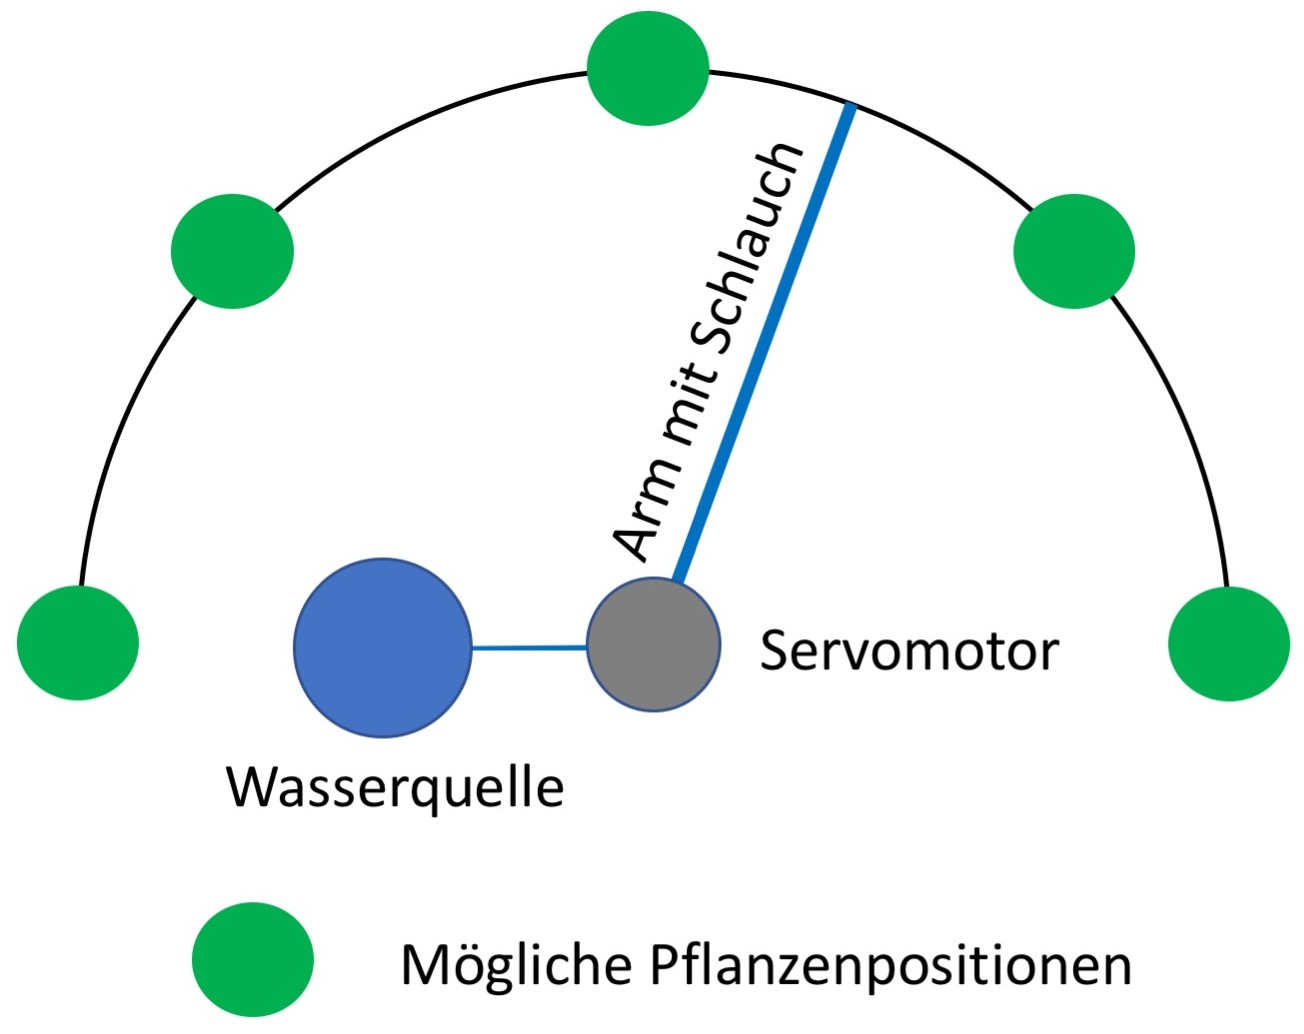
\includegraphics[width=0.6\linewidth]{Pictures/Konzept/Position}
            \caption{Anordnung der Pflanzen}
            \label{fig:position}
        \end{figure}
    
        \subsection{Codequalität}
        Die Codequalität der React Native App wird anhand des Tools \textit{ESLint} überwacht. ESLint wird mit der Konfiguration von Google genutzt und um Validierungen für React und React Native erweitert.
        Die Django-App wird mittels eines Linters auf die Einhaltung des Python-Styleguides PEP 8 validiert.
        
    \section{Implementierung}

    \subsection{Projektaufbau}
React Native bietet eine Option einfach ein neues Projekt anzulegen. Der Befehl \textit{react-native init "projectname"} geniert alle benötigten Dateien und Ordner um ein Projekt zu starten. Dies ermöglicht einen schnellen, einfachen Einstieg in React Native. Die initiale Ordnerstruktur wurde im Zuge der React Native Arbeit näher erläutert. Für größere Projekte ist diese Struktur allerdings nicht ideal. Die initial generierten Dateien \textit{index.android.js} und \textit{index.ios.js} dienen den nativen Android und iOS Apps als Ausgangspunkt. Mit dem Befehl \textit{AppRegistry} kann die App dort registriert werden. Die Dateien enthalten zu Anfang allerdings viel doppelten Code. Um die Codequalität zu verbessern und zu vereinheitlichen wurde deshalb die Ordnerstruktur für das Projekt angepasst. Ziele für die Umstrukturierung war die maximale Wiederverwendbarkeit von Code. Die Graphik \ref{lst:directory_structure} zeigt die verwendete Ordnerstruktur.

  \lstdefinestyle{tree}{
      literate=
      {├}{{\smash{\raisebox{-1ex}{\rule{1pt}{\baselineskip}}}\raisebox{0.5ex}{\rule{1ex}{1pt}}}}1 
      {─}{{\raisebox{0.5ex}{\rule{1.5ex}{1pt}}}}1 
      {└}{{\smash{\raisebox{0.5ex}{\rule{1pt}{\dimexpr\baselineskip-1.5ex}}}\raisebox{0.5ex}{\rule{1ex}{1pt}}}}1 
    }
    
    \begin{lstlisting}[style=tree]
    .
    ├── .babelrc
    ├── .buckconfig
    ├── .eslintrc.json
    ├── .flowconfig
    ├── .watchmanconfig
    ├── __tests__/
    ├── android/
    ├── app/
    ├── index.android.js
    ├── index.ios.js
    ├── ios/
    ├── node_modules/
    └── package.json
    \end{lstlisting}
    \vspace{-0.5 cm}
    \begin{listing}[H]
        \caption{Verzeichnisstruktur des React Native Projekts}
        \label{lst:directory_structure}
    \end{listing}
    
 Die Android und iOS Ordner enthalten den Nativen Code für die Apps. Die React Native Entwicklung der App befindet sich fast ausschließlich in dem Ordner \textit{app}. Die Entwicklung von Tests befindet sich in \textit{\_\_tests\_\_}. Die verwendeten Bibliotheken stehen in der \textit{package.json} Datei und deren Versionen können dort angepasst werden. Die Konfiguration des JavaScript-Compilers befindet sich in der \textit{.babelrc} Datei. Die \textit{package.json} führt die verwendeten Bibliotheken und deren Versionen auf, während die .eslintrc.json den Code-Linter konfiguriert.
 
 In der Graphik \ref{lst:app_directory_structure} sind die Unterordner des Ordners app zu sehen. Die \textit{index.js} Datei wird von den Dateien \textit{index.android.js}und \textit{index.ios.js} importiert. Der erste zu erwähnende Ordner ist \textit{components}. Dieser dient der Strukturierung von wiederverwendbaren Komponenten, wie beispielsweise Buttons. \\
 In dem Ordner \textit{config} befindet sich wiederverwendbare Styles, die so von überall her genutzt werden können. Zusätzlich befinden sich in der \textit{images.js}-Datei Pfade für die verwendeten Bilder. Damit können diese zentral verwaltet werden. Die Bilder selbst werden im Ordner \textit{images} gespeichert.\\
 Die Ordner \textit{database} und \textit{network} enthalten jeweils Module, welche die API-Aufrufe bzw. die Datenbank-Operationen implementieren und über abstrakte Methoden zur Verfügung stellen. \\
 Der \textit{redux}-Ordner beinhaltet die verschiedenen \textit{Actions}, d.h. Events, die den globalen State verändern, sowie die \textit{Reducer}, welche entscheiden, wie eine Action den globalen State verändert.
 
 Die Routen reflektieren die verschiedenen Views in der App. Die Views werden in \ref{views} näher erklärt. In dem Ordner \textit{routes} werden die Views implementiert. Hier befindet sich der Hauptteil der Implementierung der App. Die Datei \textit{router.js} ist zuständig zwischen den verschiedenen Views zu navigieren und den aktuellen View anzuzeigen. Die Datei wird von der index.js Datei importiert. Dies sorgt für eine übersichtliche Entwicklung aller Teile der App. 
 
    \begin{lstlisting}[style=tree]
    .
    ├── components
    ├── config
    ├── database
    ├── images
    ├── index.js
    ├── router.js
    ├── models
    ├── network
    ├── redux
    └── routes

    \end{lstlisting}
    \vspace{-0.5 cm}
    \begin{listing}[H]
        \caption{Inhalte des Ordners \textit{app}}
        \label{lst:app_directory_structure}
    \end{listing}
        
        
        
    \subsection{Mobile Applikation}
        
        \subsubsection{Installation}
Um das Projekt mit React native ausführen zu können, muss als erstes Node installiert sein. Zusätzlich sollte \textit{Watchman} installiert werden. Dies beobachtet Dateiänderungen und sorgt für eine bessere Performance \cite{facebook_inc._start_2017}.  Als nächstes kann mit dem Package-Manager npm das Paket \textit{react-native-cli},welches das  React Native command line interface ist, installiert werden. \\

Vor dem Ausführen der App müssen noch die benötigten Libraries installiert werden. Dazu wird im Projektordner folgender Befehl auf dem Terminal aufgerufen:
\begin{listing}[H]
    \begin{minted}{bash}
    npm install
    react-native link
    \end{minted}
    \caption{Installation der benötigten Bibliotheken}
    \label{lst:npm_linstall}
\end{listing}
Zusätzlich sind für die Bibliothek \textit{Image-Crop-Picker } noch einige manuell Schritte nötig. Dieser dient zum auswählen der Bilder in der App. In Xcode muss dafür noch unter \textit{Deployment Info} das \textit{Deployment Target} auf 8.0 gesetzt werden. Unter dem Punkt \textit{Embedded Binaries} werden die beiden Dateien \textit{RSKImageCropper.framework} und \textit{QBImagePicker.framework} noch hinzugefügt \cite{pusic_crop_2017}.

Um die App nun zu starten, sind nun je nach Zielplattform die in Listing \ref{lst:run} aufgeführten Befehle auszuführen. Dabei ist zu beachten, dass für Android das Android-SDK sowie ein gestarteter Android-Emulator vorhanden sein muss.
\begin{listing}[H]
    \begin{minted}{bash}
    react-native run-ios // Start der App auf dem iPhone-Simulator
    react-native run-android // Stat der App auf dem Android-Simulator
    \end{minted}
    \caption{Ausführen der App}
    \label{lst:run}
\end{listing}

Alternativ kann die App auch über das Xcode-Projekt im ios Ordner der App gestartet werden. Dabei kann eine iOS App nur auf dem MacOS-System gestartet werden. \cite{facebook_inc._start_2017}\\
Zum Ausführen der Android App kann außerdem Android Studio oder eine ähnliche Umgebung genutzt werden.

 
        \subsubsection{Verwendete Bibliotheken}
        
        \subsubsection*{ExNavigation}
Um eine einfache und übersichtliche  Navigation zu gewährleisten würde die Bibliothek \textit{ExNavigation} verwendet. Die Bibliothek wird im Moment in die reactjs Organisation eingebunden und in der nächsten Version unter dem Namen \textit{react-navigation} verfügbar sein \cite{Vatne_exnavigation_2017}. Die Bibliothek ermöglicht eine einfachere Navigation als die Standard React Native Navigation im Moment. Mit wenig Entwicklungsaufwand konnte so die Navigation zwischen den Views ermöglicht werden. \\

        \subsubsection*{Realm}
        Um die vom Nutzer bereitgestellten Daten, wie die ID des Microcontrollers oder die lokalen Pfade der Bilder, auch nach dem Beenden der App zu speichern, wird die Datenbank \textit{Realm} genutzt. Diese Datenbank ist speziell für mobile Geräte gedacht und die außer für React Native auch für verschiedene andere mobile Plattformen und Frameworks, wie iOS, Android, Xamarin, verfügbar ist \cite{Realm_2016}. Die Funktionen von Realm gehen dabei weit über die Möglichkeiten des React Native eigenen Key-Value-Stores hinaus und bieten eine einfachere Aufrufsemantik im Gegensatz zur SQLite-Bibliotheken, die mittels puren SQL-Befehlen arbeiten.
        Weiterhin besitzt Realm ein vielfaches der Performance anderer mobiler Datenbanken, wie anhand des öffentlich verfügbaren Benchmarks nachvollzogen werden kann \cite{Realm_Benchmark_2016}.
        
        \subsubsection*{Redux}
        \textit{Redux} ist eine Bibliothek für React (Native) zum Umgang mit globalen App-State. React und React-Native-Komponenten können Eigenschaften an Kindkomponenten weitergeben. Hierbei können auch Funktionen übergeben werden, die als Callback fungieren und es erlauben als Kindkomponente den Status von Elternkomponenten zu verändern. Dieses Vorgehen ist für kleine Applikation absolut ausreichend. Sobald Apps jedoch größer werden und mehrere Komponenten eine gemeinsame Variable teilen, deren Änderung sich auf alle Komponenten auswirkt, wird das beschriebene Vorgehen rasch unübersichtlich und komplex. Redux definiert daher einen zentralen Speicher für den App-State, der von einer Komponente durch das Auslösen eines Events geändert werden kann und dessen Änderungen automatisch an alle abhängigen Komponenten kommuniziert werden.
        
        \subsubsection*{Image-Crop-Picker}
        Diese Bibliothek übernimmt den Prozess der Auswahl eines Bildes durch den Nutzer aus der Bildergalerie des Gerätes sowie das Zuschneiden des Bildes auf das benötigte Seitenverhältnis.
        
        \subsubsection*{Fetch-Blob}
        Der Image-Crop-Picker die ausgewählten Bilder in einem temporären Verzeichnis, dessen Inhalte nach einer bestimmten Zeit automatisch gelöscht werden. Um die Löschung der Pflanzenbilder zu vermeiden, werden die Bilder daher sofort nach Auswahl in ein dauerhaftes App-Verzeichnis verschoben. \textit{Fetch-Blob} dient dazu die Dateioperationen auf Verzeichnisebene zu übernehmen. 

\subsection{Server}
    
    \subsubsection{Installation / Ausführung}
        \paragraph*{Voraussetzungen}
            \begin{itemize}
                \item Laufende Redis-Instanz
                \item Installiertes Python 3 
                \item Installiertes Python-Paketverwaltung pip
            \end{itemize}
        
        \paragraph*{Installation}\mbox{}\\
        Vor der Ausführung der Serverkomponente müssen folgende Konfigurationsdateien erstellt bzw. bearbeitet werden:
        \begin{itemize}
            \item \textit{server/watering\_of\_things.celery.py}\\
            Hier müssen die Verbindungsdetails für den Redis-Server hinterlegt werden
            \item \textit{server/watering\_of\_things/config/mqtt\_settings.py}\\
            Wie in der Datei \textit{mqtt\_settings\_example.py} zu sehen, müssen die Verbindungsdetails zum MQTT-Broker hinterlegt werden. Für Testkonfigurationen können hier auch kostenlose, öffentliche Broker genutzt werden.
        \end{itemize}
     Anschließend müssen die benötigten Abhängigkeiten installiert werden. Eine virtuelle Umgebung wird empfohlen, ist jedoch nicht zwingend nötig.
     \begin{listing}[H]
         \begin{minted}{bash}
         cd server/
         pip install -r requirements.txt
         \end{minted}
         \caption{Installieren der benötigten Frameworks / Bibliotheken}
     \end{listing}
     
     Nun folgt das initialisieren der Datenbank:
     \begin{listing}[H]
     \begin{minted}{bash}
     python3 manage.py makemigrations api
     python3 migrate
     \end{minted}
     \caption{Initialisieren der Datenbank}
      \end{listing}

 
     Anschließend kann müssen der Server gestartet werden sowie der Celery-Worker, welcher periodisch die Feuchtigkeitsmessungen über MQTT vom Microcontroller anfordert.
    
    \begin{listing}[H]
        \begin{minted}{bash}
        python3 manage.py runserver // default port
        # python3 manage.py localhost:<port>
                
        celery -B  -A watering_of_things worker -l info
        \end{minted}
        \caption{Ausführen der Web-Application}
    \end{listing}
    
    Achtung: Läuft der Server nicht auf dem Localhost, so muss er via HTTPS bereitgestellt werden, da iOS ungesicherte Verbindungen zu externen Servern unterbindet.
    
    Soll eine valide Microcontroller-ID hinterlegt werden, muss zuerst auf die Python-Shell gewechselt werden:
    \begin{listing}[H]
        \begin{minted}{bash}
        python3 manage.py shell
        \end{minted}
        \caption{Wechsel auf Python-Shell}
    \end{listing}
    Nun kann ein Microcontroller mit der gewünschten ID hinterlegt werden.
    \begin{listing}[H]
        \begin{minted}{python}
        from watering_of_things.api.models import MicroController
        MicroController('<any id>').save()
        exit()
        \end{minted}
        \caption{Hinterlegen einer validen Controller-ID}
    \end{listing}

    \subsubsection{Security}
    Die Sicherheit der Verbindung wird zum einen durch die Verwendung von HTTPS sichergestellt. Zum anderen sind die Controller-IDs 32-stellige Tokens, welche nur dem Server und dem Eigentümer des Controllers bekannt sind. Diese dienen neben der Identifizierung weiterhin zur Tokenauthentifizierung für die Kommunikation zwischen App und REST Api.
    
\subsection{Microcontroller}
    \subsubsection{Schaltplan}
    
    \subsubsection{Installation / Ausführung}
    
    \paragraph*{Voraussetzung}
    \begin{itemize}
        \item Installierte Arduino IDE
        \item Treiber für den NodeMCU 1.0
    \end{itemize}

    \paragraph*{Installation}\mbox{}\\
    Zuerst muss die Unterstützung für den NodeMCU durch die Arduino IDE installiert werden. Dazu unter \textit{Werkzeuge --> Board --> Boardverwalter} das Paket \textit{esp8266} von der \textit{ESP8266 Community} installiert werden sowie unter \textit{Werkzeuge --> Board} das Board \textit{NodeMCU 1.0} ausgewählt werden. Nachdem Verbinden des Boards muss der richtige Port unter \textit{Werkzeuge --> Port} ausgewählt werden. Weiter muss die Library \textit{PubSubClient} von \textit{Nick O'Leary} mittels \textit{Sketch --> Bibliothek einbinden --> Bibliotheken verwalten} installiert werden.
    
    Anschließend müssen noch die Controller-ID sowie die Verbindungseinstellungen konfiguriert werden:
    \begin{itemize}
        \item ID.h\\
        ID des Controllers, welche ebenfalls auf dem Server hinterlegt sein muss
        \item WifiConfig.h\\
        Name und Passwort des Wlans mit dem sicher Controller verbinden soll
        \item MqttConfig.h\\
        Verbindungsdetails für den MQTT-Broker
    \end{itemize}

    Anschließend kann der Code mittels des Buttons \textit{Hochladen} auf den Controller übertragen werden. Damit sowohl Pumpe als auch Servo-Motor funktionieren muss die Platine mit einer 12V-Stromversorgung verbunden sein.
    
     
    
   	\section{Résumé}
Mit dem Einsatz von WateringOfThings kann der Nutzer nun seine Pflanzen auch längere Zeit über alleine lassen, ohne auf eine ideale Bewässerung der Pflanzen verzichten zu müssen. Das Projekt stellt dabei eine Verknüpfung von Webtechnologien und Internet of Things dar. Dabei wurden zum einen eine native Smartphone-Applikation geschrieben, die sowohl auf Android als auch iOS lauffähig ist. Zum anderen wurde mithilfe von Django ein Web-API umgesetzt, die die Kommunikation mit den Hardwarekomponenten übernimmt sowie die gesammelten Daten zentral verwaltet und bereitstellt. Darüber hinaus wurde eine eigene Hardwarekomponente, beginnend von der Auswahl der benötigten Teile bis hin zur Umsetzung eines eigenen Platinenlayouts, konzeptioniert und in die Gesamtarchitektur mittels des leichtgewichtigen MQTT-Protokolls eingebunden. Im Zusammenspiel setzen diese drei Komponenten alle in Kapitel \ref{sec:usecases} beschriebenen Use Cases um. Aufgrund des Nutzen von WateringOfThings wird eine Fortführung des Projektes angestrebt. Dafür kommen folgende Features in Frage:
\begin{itemize}
    \item Hinzufügen eines weiteren Sensors, um den Nutzer über Fehlfunktionen zu benachrichtigen
    \item Weitere Sensoren (Licht, Temperatur), um die Bewässerung zu automatisieren
    \item Bündelung der Hardware in einem sich selbst bewässernden Blumentopf
    \item Push-Notifications, um den Nutzer über zu trockene Pflanzen zu informieren
    \item Möglichkeit mehrere Hardwarekomponenten pro App zu verwalten
    \item Nutzertests um die UI nutzerfreundlicher zu gestalten
    \item Visualisierung des Verlaufs der Feuchtigkeit einer Pflanze
    \item Hinzufügen weiterer Sensoren, um den Düngebedarf der Blumenerde festzustellen
\end{itemize}


    \clearpage
	\printbibliography %Literaturverzeichnis
\end{document}
